\documentclass[]{report}
\usepackage{hyperref}
\usepackage{graphicx}
\hypersetup{colorlinks=true, linkcolor=black, urlcolor=blue}

\begin{document}

\title{{\Huge\textit{myTaxiService}}\\{\Large Integration test plan document}}
\author{Belluschi Marco 791878, Cerri Stefano 849945, Di Febbo Francesco 852389}

\maketitle

\tableofcontents

\chapter{Introduction}

	\section{Revision history}
	In the following are listed the differences between versions:
\begin{enumerate}
	\item Document creation
\end{enumerate}

	\section{Purpose and scope}
	\subsection{Purpose}
	This is the \textit{Project Plan} (\textbf{PP}) for \textit{myTaxiService}.
	Its purpose is to evaluate time and resources necessary to develop the entire \textit{myTaxiService} system, including mobile and web applications.\\
	To do so, the \textbf{Function Points} measurement and the \textbf{COCOMO} model have been used, comparing the results with the system size and the implementation time.

\subsection{Scope}
	As more widely explained both in the RASD and in the DD, myTaxiService
	is a taxi service for a large city. The main goals of the system
	are:
	\begin{itemize}
		\item simplify the access of passengers to the service;
		\item guarantee a fair management of taxi queues.
	\end{itemize}
	See the two aforementioned documents for further explanations.

	\section{List of definitions and abbreviations}
	\paragraph{Definitions}
	\begin{itemize}
		\item Function Point: unit of measurement that expresses the amount of business functionality an information system (as a product) provides to a user compared to software size; costs (in dollars or hours) are calculated from past projects
		\item COCOMO Model: algorithmic software cost estimation model that uses a basic regression formula with parameters derived from historical project data and current/future project characteristics
		\item User: person that uses the service applications
		\item Passenger: passenger registered to the service
		\item Taxi driver: taxi driver registered to the service
		\item Mobile App: \textit{myTaxiService} mobile application
		\item Web App: \textit{myTaxiService} web application
		\item System: the union of software and hardware to be developed and implemented
	\end{itemize}

\paragraph{Acronyms}
	\begin{itemize}
		\item PP: Project Plan
		\item RASD: Requirements Analysis and Specification Document
		\item DD: Design Document
		\item ITPD: Integration Test Plan Document
		\item FP: Function Point
		\item COCOMO: COnstructive COst MOdel
		\item SLOC: Source Line Of Code
		\item KSLOC: 1000 SLOCs
		\item EAF: Effort Adjustement Factor
		\item ILF: Internal Logic File
		\item EIF: External Interface File
		\item EI: External Input
		\item EO: External Output
		\item EQ: External Inquiry
	\end{itemize}

	\section{List of reference documents}
	\begin{itemize}
	\item Software Engineering 2 Project AA 2015/2016: Project Description And Rules
	\item Software Engineering 2 Project AA 2015/2016: Assignments 1 and 2 (RASD and DD) 
	
\end{itemize}

\chapter{Integration strategy}

	\section{Entry criteria}
	
The main entry condition for this phase is that each of the system components low level functions has been previously subjected to a unit test process.
The documentation of all classes and functions must be written in JavaDoc. In particular, the public interfaces of each class and module should be well specified; where necessary with the formal specification language JML.



	\section{Elements to be integrated}
	myTaxiService, as shown in Design Document, is a three-tier system:
\begin{itemize}
	\item DBMS
	\item myTaxiService server
	\item Client application
\end{itemize}
Each tier is composed by interacting modules:
\begin{enumerate}
	\item Application (web/mobile)
	\item Data manager
	\item Account manager
	\item Ride manager
	\item Taxi queues
	\item Map services
	\item Notification		
\end{enumerate}


	\section{Integration testing strategy}
	The integration testing strategy, conducted in this project, is a \textit{bottom-up} approach. This strategy tests the lower level components and start testing a way upwards to higher level components. The advantage of this strategy is that it's easier to maintain code, smaller modules have unit tests and there is a clearer structure of how to do things. The disadvantage is that when releasing a prototype it's impossible to see a working prototype until nearly all the program has been completed so that may take a long time before this happens. There may be a lot of errors later on regarding the GUI and programming later on.


	\section{Sequence of component/function integration}
	\input{integration_strategy/function_integration.tex}
	
		\subsection{Software integration sequence}
		The following diagram illustrates the integration sequence of the various components, following the integration testing strategy described above. This means that in each subsystem, components are integrated starting from the most independent to the less independent, in order to prompt the chosen approach and improving modularity.

\begin{center}
	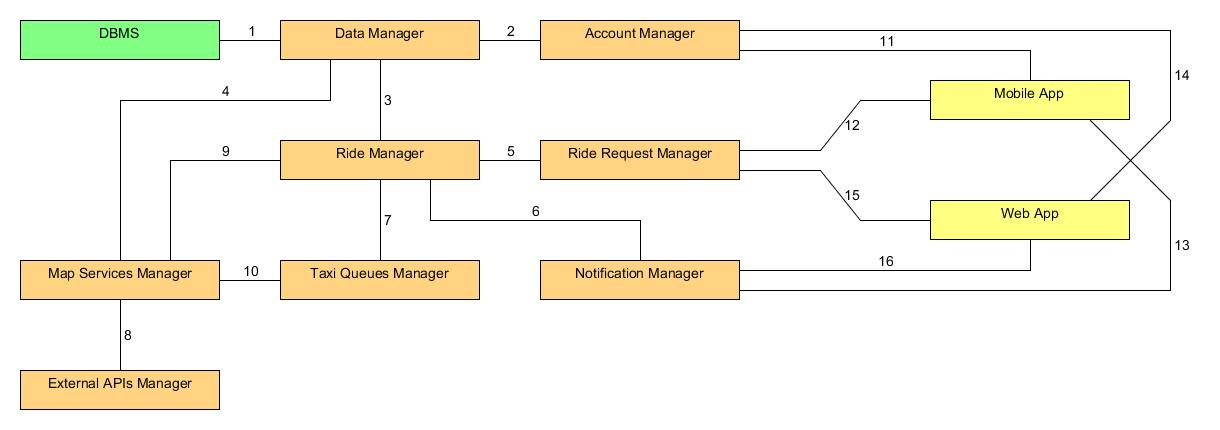
\includegraphics[width=\textwidth]{diagrams/SoftwareIntegrationDiagram.jpg}
\end{center}
	
		\subsection{Subsystem integration sequence}
		The following diagram illustrates the integration sequence of the various subsystems, following the integration testing strategy described above. In particular, the Server Database is integrated before the Client, because the former does not need an actual functioning system in order to be tested efficiently, contrary to the latter.

\begin{center}
	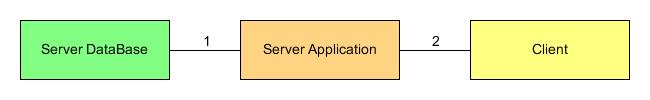
\includegraphics[width=\textwidth]{diagrams/SubsystemsIntegrationDiagram.jpg}
\end{center}

\chapter{Individual steps and test description}
\section{Individual Step and Test Description}
  
   \subsection{Test Case I1}
   \begin{table}[ht!]
   	\begin{tabular*}{16cm}{ll}
   		\hline
   		\textbf{Test Item(s)} & Data Manager $ \longleftrightarrow $ DBMS  \\
   		\hline
   		\textbf{Input Specification} & \pbox{20cm}{Queries on the DBMS for the Table User, Passenger, Taxi Driver and Ride}\\
   		\hline
   		\textbf{Output Specification} & \pbox{20cm}{The queries return the expected results}\\
   		\hline
   		\textbf{Environmental Needs} &  \pbox{20cm}{Glassfish Server, a test Database}\\
   		\hline
   		\textbf{Purpose} & \pbox{20cm}{Verify that the typical queries to the DBMS works} \\
   		\hline
   	\end{tabular*}
   \end{table}
   
    \subsection{Test Case I2}
    \begin{table}[ht!]
    	\begin{tabular*}{16cm}{ll}
    		\hline
    		\textbf{Test Item(s)} & Data Manager $ \longleftrightarrow $ Account Manager   \\
    		\hline
    		\textbf{Input Specification} & \pbox{20cm}{A set of methods calls on Data Manager to retrieve user information }\\
    		\hline
    		\textbf{Output Specification} & \pbox{20cm}{Check that the user information are correct }\\
    		\hline
    		\textbf{Environmental Needs} &  \pbox{20cm}{Glassfish Server, a test Database, I1 successful}\\
    		\hline
    		\textbf{Purpose} & \pbox{20cm}{Verify that the user information are retrieved from the Data Manager} \\
    		\hline
    	\end{tabular*}
    \end{table}
    
    \newpage
     \subsection{Test Case I3}
     \begin{table}[ht!]
     	\begin{tabular*}{16cm}{ll}
     		\hline
     		\textbf{Test Item(s)} & Data Manager $ \longleftrightarrow $  Ride Manager \\
     		\hline
     		\textbf{Input Specification} & \pbox{20cm}{A set of methods calls on Data Manager to retrieve reserved \\ ride information}\\
     		\hline
     		\textbf{Output Specification} & \pbox{20cm}{Check that the reserved ride information are correct}\\
     		\hline
     		\textbf{Environmental Needs} &  \pbox{20cm}{Glassfish Server, a test Database, I1 successful}\\
     		\hline
     		\textbf{Purpose} & \pbox{20cm}{Verify that the reserved ride information are retrieved from \\ the Data Manager} \\
     		\hline
     	\end{tabular*}
     \end{table}
     
      \subsection{Test Case I4}
      \begin{table}[ht!]
      	\begin{tabular*}{16cm}{ll}
      		\hline
      		\textbf{Test Item(s)} & Data Manager $ \longleftrightarrow $ Map Service Manager  \\
      		\hline
      		\textbf{Input Specification} & \pbox{20cm}{A set of methods calls on Data Manager to retrieve zone information }\\
      		\hline
      		\textbf{Output Specification} & \pbox{20cm}{Check that the zone information are correct}\\
      		\hline
      		\textbf{Environmental Needs} &  \pbox{20cm}{Glassfish Server, a test Database, I1 successful}\\
      		\hline
      		\textbf{Purpose} & \pbox{20cm}{Verify that the zone information are retrieved from the Data Manager} \\
      		\hline
      	\end{tabular*}
      \end{table}
      
       \subsection{Test Case I5}
       \begin{table}[ht!]
       	\begin{tabular*}{16cm}{ll}
       		\hline
       		\textbf{Test Item(s)} & Ride Request Manager $ \longleftrightarrow $ Ride Manager \\
       		\hline
       		\textbf{Input Specification} & \pbox{20cm}{A typical set of methods calls on Ride Manager in order to create a Ride}\\
       		\hline
       		\textbf{Output Specification} & \pbox{20cm}{Check if the correct Ride is created with the information from \\ Ride Request Manager}\\
       		\hline
       		\textbf{Environmental Needs} &  \pbox{20cm}{I2 successful}\\
       		\hline
       		\textbf{Purpose} & \pbox{20cm}{Create a Ride from a typical Ride Request} \\
       		\hline
       	\end{tabular*}
       \end{table}
       
        \subsection{Test Case I6}
        \begin{table}[ht!]
        	\begin{tabular*}{16cm}{ll}
        		\hline
        		\textbf{Test Item(s)} & Ride Manager $ \longleftrightarrow $ Notification Manager  \\
        		\hline
        		\textbf{Input Specification} & \pbox{20cm}{A set of methods calls in order to create a notification}\\
        		\hline
        		\textbf{Output Specification} & \pbox{20cm}{Check if the correct notification is created}\\
        		\hline
        		\textbf{Environmental Needs} &  \pbox{20cm}{I2 and I5 successful}\\
        		\hline
        		\textbf{Purpose} & \pbox{20cm}{Verify that the Notification Manager create the notification from the Ride Manager} \\
        		\hline
        	\end{tabular*}
        \end{table}
       
 \newpage
        
         \subsection{Test Case I7}
         \begin{table}[ht!]
         	\begin{tabular*}{16cm}{ll}
         		\hline
         		\textbf{Test Item(s)} & Ride Manager $ \longleftrightarrow $ Taxi Queues Manager  \\
         		\hline
         		\textbf{Input Specification} & \pbox{20cm}{A set of methods calls on Taxi Queues Manager }\\
         		\hline
         		\textbf{Output Specification} & \pbox{20cm}{Check if an available Taxi Driver is returned}\\
         		\hline
         		\textbf{Environmental Needs} &  \pbox{20cm}{I2 and I6 successful}\\
         		\hline
         		\textbf{Purpose} & \pbox{20cm}{Retrieve an available Taxi Driver} \\
         		\hline
         	\end{tabular*}
         \end{table}
   
    \subsection{Test Case I8}
    \begin{table}[ht!]
    	\begin{tabular*}{16cm}{ll}
    		\hline
    		\textbf{Test Item(s)} & Map Services Manager $ \longleftrightarrow $ External APIs Manager  \\
    		\hline
    		\textbf{Input Specification} & \pbox{20cm}{Create a typical set of methods calls by Map Services Manager \\ on External APIs Manager}\\
    		\hline
    		\textbf{Output Specification} & \pbox{20cm}{Check that all the methods of External APIs Manager produce \\ the expected results}\\
    		\hline
    		\textbf{Environmental Needs} &  \pbox{20cm}{N/A}\\
    		\hline
    		\textbf{Purpose} & \pbox{20cm}{Verify that the External APIs Manager works with the \\ Map Services Manager} \\
    		\hline
    	\end{tabular*}
    \end{table}
    
         
   \subsection{Test Case I9}
   \begin{table}[ht!]
   	\begin{tabular*}{16cm}{ll}
   		\hline
   		\textbf{Test Item(s)} & Ride Manager $ \longleftrightarrow $ Map Services Manager  \\
   		\hline
   		\textbf{Input Specification} & \pbox{20cm}{A set of methods calls on Map Services Manager}\\
   		\hline
   		\textbf{Output Specification} & \pbox{20cm}{Verify that the returned route is the correct one}\\
   		\hline
   		\textbf{Environmental Needs} &  \pbox{20cm}{I5 and I8 successful}\\
   		\hline
   		\textbf{Purpose} & \pbox{20cm}{Compute the optimal route} \\
   		\hline
   	\end{tabular*}
   \end{table}

   \subsection{Test Case I10}
   \begin{table}[ht!]
   	\begin{tabular*}{16cm}{ll}
   		\hline
   		\textbf{Test Item(s)} & Taxi Queues Manager  $ \longleftrightarrow $ Map Services Manager    \\
   		\hline
   		\textbf{Input Specification} & \pbox{20cm}{A set of methods calls on Map Services Manager}\\
   		\hline
   		\textbf{Output Specification} & \pbox{20cm}{Verify that the position of the Taxi Driver is correct}\\
   		\hline
   		\textbf{Environmental Needs} &  \pbox{20cm}{I2 and I8 successful}\\
   		\hline
   		\textbf{Purpose} & \pbox{20cm}{Retrieve the position of a Taxi Driver in a Taxi Queue} \\
   		\hline
   	\end{tabular*}
   \end{table}

  
   \newpage
  
  \subsection{Test Case I11}
  \begin{table}[ht!]
  	\begin{tabular*}{16cm}{ll}
  		\hline
  		\textbf{Test Item(s)} & Account Manager $ \longleftrightarrow $   Mobile App\\
  		\hline
  		\textbf{Input Specification} & \pbox{20cm}{Create a typical set of methods calls performed by Mobile App \\ on Account Manager}\\
  		\hline
  		\textbf{Output Specification} & \pbox{20cm}{Check if the methods calls mentioned in Input Specification \\ produce the expected results}\\
  		\hline
  		\textbf{Environmental Needs} &  \pbox{20cm}{A device that can run Mobile App}\\
  		\hline
  		\textbf{Purpose} & \pbox{20cm}{Verify if Account Manager can handle correctly \\ Mobile App methods calls} \\
  		\hline
  	\end{tabular*}
  \end{table}
  
  \subsection{Test Case I12}
  \begin{table}[ht!]
  	\begin{tabular*}{16cm}{ll}
  		\hline
  		\textbf{Test Item(s)} & Ride Request Manager $ \longleftrightarrow $   Mobile App\\
  		\hline
  		\textbf{Input Specification} & \pbox{20cm}{Create a typical set of methods calls performed by Mobile App \\ on Ride Request Manager}\\
  		\hline
  		\textbf{Output Specification} & \pbox{20cm}{Check if the methods calls mentioned in Input Specification \\ produce the expected results}\\
  		\hline
  		\textbf{Environmental Needs} &  \pbox{20cm}{A device that can run Mobile App}\\
  		\hline
  		\textbf{Purpose} & \pbox{20cm}{Verify if Ride Request Manager can handle correctly \\ Mobile App methods calls} \\
  		\hline
  	\end{tabular*}
  \end{table}
  
  
  \subsection{Test Case I13}
  \begin{table}[ht!]
    \begin{tabular*}{16cm}{ll}
	\hline
	\textbf{Test Item(s)} & Notification Manager $ \longleftrightarrow $   Mobile App\\
	\hline
	\textbf{Input Specification} & \pbox{20cm}{Create a typical set of methods calls performed by Notification Manager \\ on Mobile App}\\
	\hline
	\textbf{Output Specification} & \pbox{20cm}{Check if the methods calls mentioned in Input Specification \\ produce the expected results}\\
	\hline
	\textbf{Environmental Needs} &  \pbox{20cm}{A device that can run Mobile App}\\
	\hline
	\textbf{Purpose} & \pbox{20cm}{Verify if Mobile App can handle
		correctly Notification Manager \\ methods calls} \\
	\hline
    \end{tabular*}
  \end{table}
  
  \newpage 
  \subsection{Test Case I14}
  \begin{table}[ht!]
  	\begin{tabular*}{16cm}{ll}
  		\hline
  		\textbf{Test Item(s)} & Account Manager $ \longleftrightarrow $   Web App\\
  		\hline
  		\textbf{Input Specification} & \pbox{20cm}{Create a typical set of methods calls performed by Web App \\ on Account Manager}\\
  		\hline
  		\textbf{Output Specification} & \pbox{20cm}{Check if the methods calls mentioned in Input Specification \\ produce the expected results}\\
  		\hline
		\textbf{Environmental Needs} &  \pbox{20cm}{A device that can run Web App}\\
  		\hline
  		\textbf{Purpose} & \pbox{20cm}{Verify if Account Manager can handle correctly \\ Web App methods calls} \\
  		\hline
  	\end{tabular*}
  \end{table}
  
      
      \subsection{Test Case I15}
      \begin{table}[ht!]
      	\begin{tabular*}{16cm}{ll}
      		\hline
      		\textbf{Test Item(s)} & Ride Request Manager $ \longleftrightarrow $   Web App\\
      		\hline
      		\textbf{Input Specification} & \pbox{20cm}{Create a typical set of methods calls performed by Web App \\ on Ride Request Manager}\\
      		\hline
      		\textbf{Output Specification} & \pbox{20cm}{Check if the methods calls mentioned in Input Specification \\produce the expected results}\\
		    \hline
			\textbf{Environmental Needs} &  \pbox{20cm}{A device that can run Web App}\\
			\hline
      		\textbf{Purpose} & \pbox{20cm}{Verify if Ride Request Manager can handle correctly \\ Web App methods calls} \\
      		\hline
      	\end{tabular*}
      \end{table}
      
  
  
  \subsection{Test Case I16}
  \begin{table}[ht!]
  	\begin{tabular*}{16cm}{ll}
  		\hline
  		\textbf{Test Item(s)} & Notification Manager $ \longleftrightarrow $   Web App\\
  		\hline
  		\textbf{Input Specification} & \pbox{20cm}{Create a typical set of methods calls performed by Notification \\ on Web App}\\
  		\hline
  		\textbf{Output Specification} & \pbox{20cm}{Check if the methods calls mentioned in Input Specification \\ produce the expected results}\\
  		\hline
		\textbf{Environmental Needs} &  \pbox{20cm}{A device that can run Web App}\\
  		\hline
  		\textbf{Purpose} & \pbox{20cm}{Verify if Web App can handle correctly Notification methods calls} \\
  		\hline
  	\end{tabular*}
  \end{table}

   \subsection{Test Case SI1}
   \begin{table}[ht!]
   	\begin{tabular*}{16cm}{ll}
   		\hline
   		\textbf{Test Item(s)} & Server Database $ \longleftrightarrow $ Server Application  \\
   		\hline
   		\textbf{Input Specification} & \pbox{20cm}{Queries on the DBMS for the Table User, Passenger, Taxi Driver and Ride}\\
   		\hline
   		\textbf{Output Specification} & \pbox{20cm}{The queries return the expected results}\\
   		\hline
   		\textbf{Environmental Needs} &  \pbox{20cm}{Glassfish Server, a test Database}\\
   		\hline
   		\textbf{Purpose} & \pbox{20cm}{Verify that the typical queries to the DBMS works} \\
   		\hline
   	\end{tabular*}
   \end{table}
   
   
   \subsection{Test Case S2}
   \begin{table}[ht!]
   	\begin{tabular*}{16cm}{ll}
   		\hline
   		\textbf{Test Item(s)} & Server Application $ \longleftrightarrow $ Client  \\
   		\hline
   		\textbf{Input Specification} & \pbox{20cm}{A set of methods calls on both Server Application and Client }\\
   		\hline
   		\textbf{Output Specification} & \pbox{20cm}{Check that the methods calls mentioned in Input Specification produce \\ the expected results }\\
   		\hline
   		\textbf{Environmental Needs} &  \pbox{20cm}{Glassfish Server, a test Database}\\
   		\hline
   		\textbf{Purpose} & \pbox{20cm}{Verify that the interaction between Server Application and Client works} \\
   		\hline
   	\end{tabular*}
   \end{table}   


\chapter{Tools and test equipment required}
This section describes the tools required to perform the integration testing plan described previously.
Following the validation and verification model, it is possible to perform different tests on components.

\begin{itemize}
	\item \textbf{jUnit}: is a unit testing framework for the Java programming language. Each individual units of source code, sets of one or more computer program modules together with associated control data, usage procedures, and operating procedures, are tested to determine whether they are fit for use.
	\item \textbf{Mockito}: is an open source testing framework for Java that allows the creation of test double objects (mock objects) in automated unit tests. It allows to abstract dependencies and have predictable results; to check that the interaction between the testee and the mock is correct. 
	\item \textbf{Arquillian}: a test framework that can be used to perform testing inside a remote or embedded container, or deploy an archive to a container so the test can interact as a remote client.
	\item \textbf{Apache JMeter}: is designed to load test functional behaviour and measure performance of a variety of services, with a focus on web applications
\end{itemize}

\chapter{Program stubs and test data required}
This section describes the specification of stubs and drivers needed to replace the part of software components that still don't exist and test the others. This is necessary to perform the integration steps.
DBMS should contain sample data in order to perform proper test cases. 
In early development, web and mobile applications are replaced by stubs to test the client connection. These stubs should provide sample data to correctly simulate real-life conditions. 
During development some components may not be available yet for integration test, thus they will be replaced by drivers.

\appendix

\chapter{Appendix}

	\section{Software and tool used}
	\begin{itemize}
	\item TeXstudio \url{http://www.texstudio.org/}: to redact and to format this document	
\end{itemize}

	\section{Working hours}
	This is the time spent for redact the document
\begin{itemize}
	\item Belluschi Marco:  10 hours
	\item Cerri Stefano:  10 hours
	\item Di Febbo Francesco: 10 hours
\end{itemize}

\end{document}
       
